\documentclass[aspectratio=169]{../latex_main/tntbeamer}  % you can pass all options of the beamer class, e.g., 'handout' or 'aspectratio=43'
\usepackage{dsfont}
\usepackage{bm}
\usepackage[english]{babel}
\usepackage[T1]{fontenc}
%\usepackage[utf8]{inputenc}
\usepackage{graphicx}
\graphicspath{ {./figures/} }
\usepackage{algorithm}
\usepackage[ruled,vlined,algo2e,linesnumbered]{algorithm2e}
\usepackage{hyperref}
\usepackage{booktabs}
\usepackage{mathtools}

\usepackage{amsmath,amssymb}

\DeclareMathOperator*{\argmax}{arg\,max}
\DeclareMathOperator*{\argmin}{arg\,min}

\usepackage{amsbsy}
\newcommand{\vect}[1]{\bm{#1}}
%\newcommand{\vect}[1]{\boldsymbol{#1}}

\usepackage{pgfplots}
\pgfplotsset{compat=1.16}
\usepackage{tikz}
\usetikzlibrary{trees} 
\usetikzlibrary{shapes.geometric}
\usetikzlibrary{positioning,shapes,shadows,arrows,calc,mindmap}
\usetikzlibrary{positioning,fadings,through}
\usetikzlibrary{decorations.pathreplacing}
\usetikzlibrary{intersections}
\pgfdeclarelayer{background}
\pgfdeclarelayer{foreground}
\pgfsetlayers{background,main,foreground}
\tikzstyle{activity}=[rectangle, draw=black, rounded corners, text centered, text width=8em]
\tikzstyle{data}=[rectangle, draw=black, text centered, text width=8em]
\tikzstyle{myarrow}=[->, thick, draw=black]

% Define the layers to draw the diagram
\pgfdeclarelayer{background}
\pgfdeclarelayer{foreground}
\pgfsetlayers{background,main,foreground}

% Requires XeLaTeX or LuaLaTeX
%\usepackage{unicode-math}

\usepackage{fontspec}
%\setsansfont{Arial}
\setsansfont{RotisSansSerifStd}[ 
Path=../latex_main/fonts/,
Extension = .otf,
UprightFont = *-Regular,  % or *-Light
BoldFont = *-ExtraBold,  % or *-Bold
ItalicFont = *-Italic
]
\setmonofont{Cascadia Mono}[
Scale=0.8
]

% scale factor adapted; mathrm font added (Benjamin Spitschan @TNT, 2021-06-01)
%\setmathfont[Scale=1.05]{Libertinus Math}
%\setmathrm[Scale=1.05]{Libertinus Math}

% other available math fonts are (not exhaustive)
% Latin Modern Math
% XITS Math
% Libertinus Math
% Asana Math
% Fira Math
% TeX Gyre Pagella Math
% TeX Gyre Bonum Math
% TeX Gyre Schola Math
% TeX Gyre Termes Math

% Literature References
\newcommand{\lit}[2]{\href{#2}{\footnotesize\color{black!60}[#1]}}

%%% Beamer Customization
%----------------------------------------------------------------------
% (Don't) Show sections in frame header. Options: 'sections', 'sections light', empty
\setbeamertemplate{headline}{empty}

% Add header logo for normal frames
\setheaderimage{
	% 
\includegraphics[height=\logoheight]{figures/TNT_darkv4.pdf}
	
\includegraphics[height=\logoheight]{../latex_main/figures/luh_logo_rgb_0_80_155.pdf}
	% 
\includegraphics[height=\logoheight]{figures/logo_tntluh.pdf}
}

% Header logo for title page
\settitleheaderimage{
	% 
\includegraphics[height=\logoheight]{figures/TNT_darkv4.pdf}
	
\includegraphics[height=\logoheight]{../latex_main/figures/luh_logo_rgb_0_80_155.pdf}
	% 
\includegraphics[height=\logoheight]{figures/logo_tntluh.pdf}
}

% Title page: tntdefault 
\setbeamertemplate{title page}[tntdefault]  % or luhstyle
% Add optional title image here
%\addtitlepageimagedefault{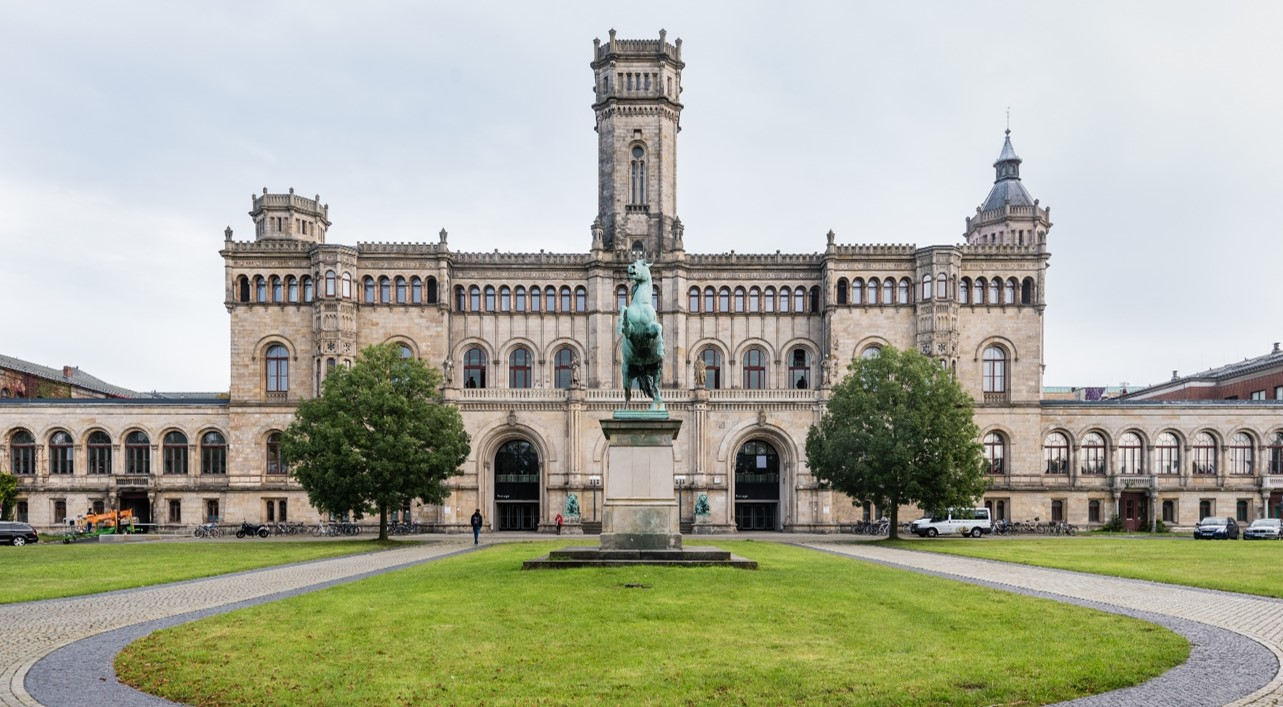
\includegraphics[width=0.65\textwidth]{figures/luh_default_presentation_title_image.jpg}}

% Title page: luhstyle
% \setbeamertemplate{title page}[luhstyle]
% % Add optional title image here
% \addtitlepageimage{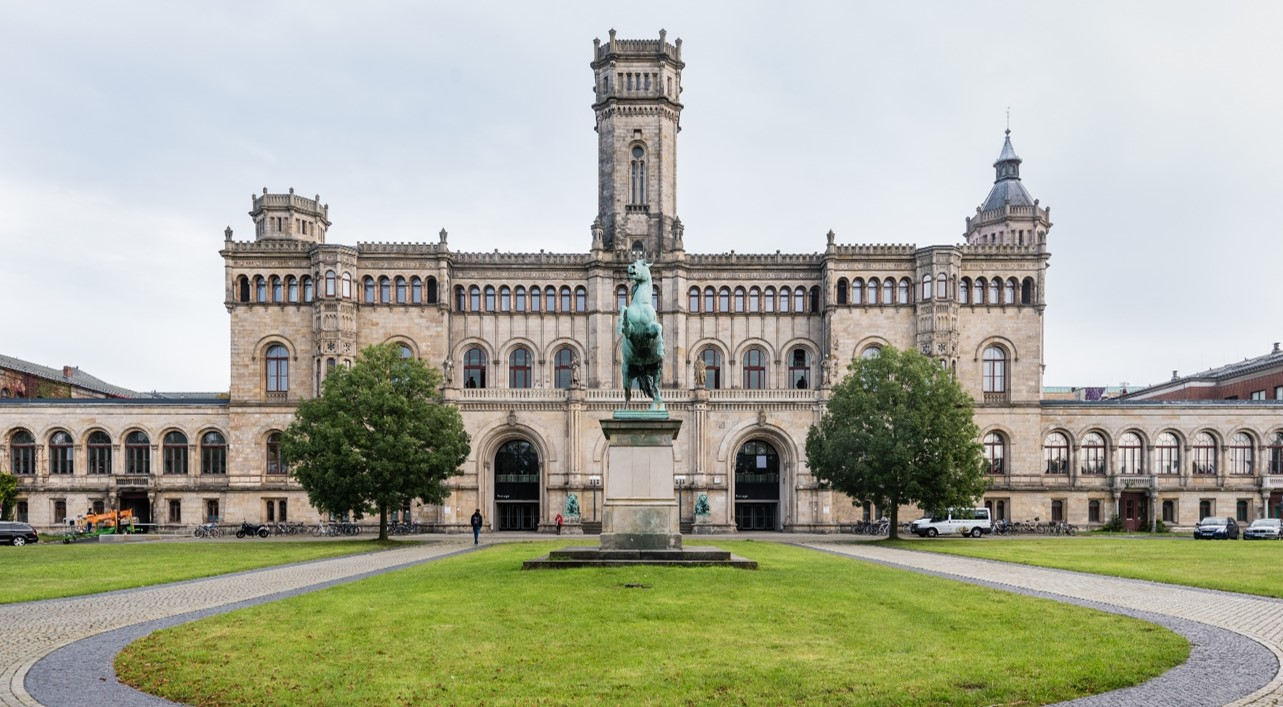
\includegraphics[width=0.75\textwidth]{figures/luh_default_presentation_title_image.jpg}}

\author[Abedjan \& Lindauer]{Ziawasch Abedjan \& Marius Lindauer\\[1em]
	
\includegraphics[height=\logoheight]{../latex_main/figures/luh_logo_rgb_0_80_155.pdf}\qquad
	
\includegraphics[height=\logoheight]{../latex_main/figures/DBIS_Kurzlogo.png}\qquad

\includegraphics[height=\logoheight]{../latex_main/figures/TNT_darkv4}\qquad

\includegraphics[height=\logoheight]{../latex_main/figures/L3S.jpg}	}
\date{Summer Term 2022; \hspace{0.5em} {
\includegraphics[height=1.5em]{../latex_main/figures/Cc-by-nc-sa_icon.svg.png}}; based on \href{https://ds100.org/fa21/}{[DS100]}
}


%%% Custom Packages
%----------------------------------------------------------------------
% Create dummy content
\usepackage{blindtext}

% Adds a frame with the current page layout. Just call \layout inside of a frame.
\usepackage{layout}


%%% Macros
%\renewcommand{\vec}[1]{\mathbf{#1}}
% \usepackage{bm}
%\let\vecb\bm

\title[Introduction]{DS: Pandas, Part 1}
\subtitle{Introduction to Pandas syntax and operators}

\graphicspath{ {./figure/} }
%\institute{}


\begin{document}
	
	\maketitle
	
	\begin{frame}{ Goals For This Lecture}
	   \begin{itemize}
	       \item Introduce Pandas, with emphasis on:
	       \begin{itemize}
	           \item A mental model of DataFrames - linking to statistics.
	           \item Key Data Structures (data frames, series, indices).
	           \item How to index into these structures.
	           \item How to read files to create these structures.
	           \item Other basic operations on these structures.
	       \end{itemize}
	       \item Will go through quite a lot of the language without full explanations. 
	       \begin{itemize}
	           \item We expect you to fill in the gaps on homeworks, labs, projects, and through your own experimentation.
	       \end{itemize}
	       \item Solve some very basic data science problems using Jupyter/pandas.
	   \end{itemize}
	\end{frame}
	
	\begin{frame}{Data Frames: a high-level, statistical perspective}
	    
	\end{frame}
	
	\begin{frame}{The world, a statistician's view }
	    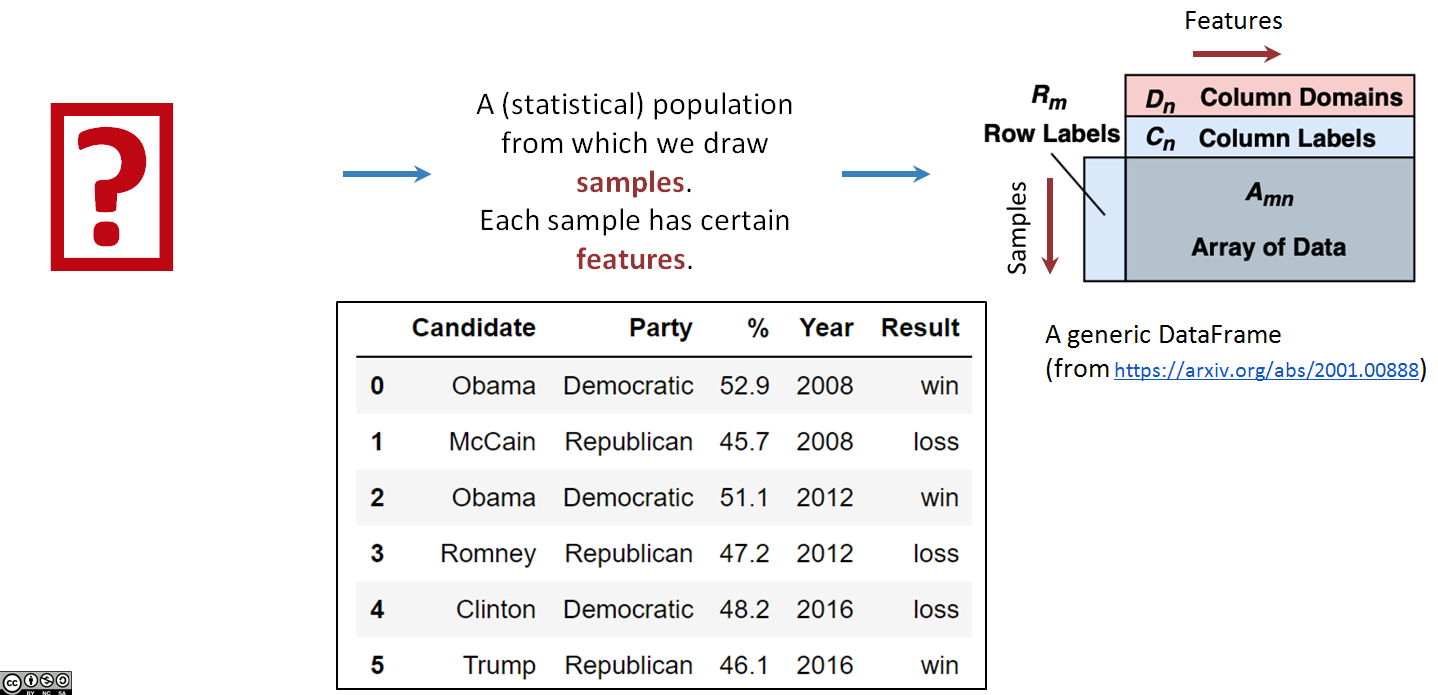
\includegraphics[scale=.36]{Bild1}
	\end{frame}
	
	\begin{frame}{Connecting with SQL: dataframes and relational ideas}
	      \begin{columns}
	        \begin{column}{.4\textwidth}
	                  \begin{figure}
	                            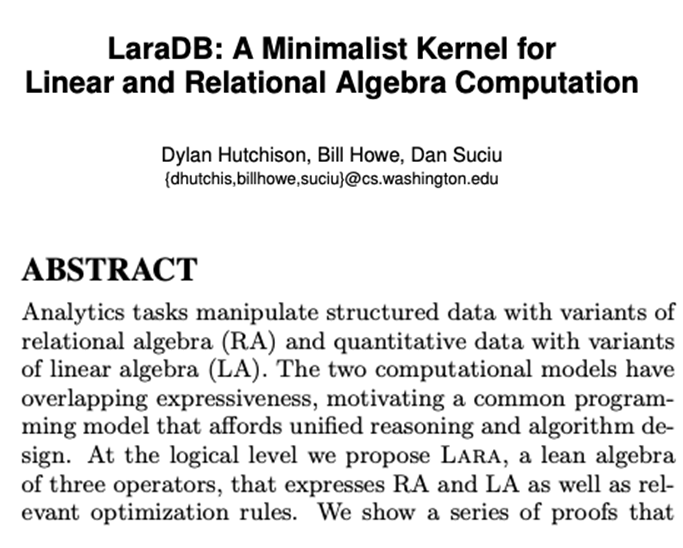
\includegraphics[scale=.3]{Bild2}  
	                  \end{figure}
	                  \url{https://arxiv.org/abs/1703.07342}
	        \end{column}
	        
	        
	        \begin{column}{.4\textwidth}
	                  \begin{itemize}
	                      \item Statistical modeling ultimately involves lots of linear algebra manipulations.
	                      \item The Relational Algebra that underlies databases (SQL) can be connected with Linear Algebra ideas.
	                  \end{itemize}
	        \end{column}
	        
	      \end{columns}
	      
	        
	       
	\end{frame}
	
	\begin{frame}{Connecting with SQL: dataframes and relational ideas}
	       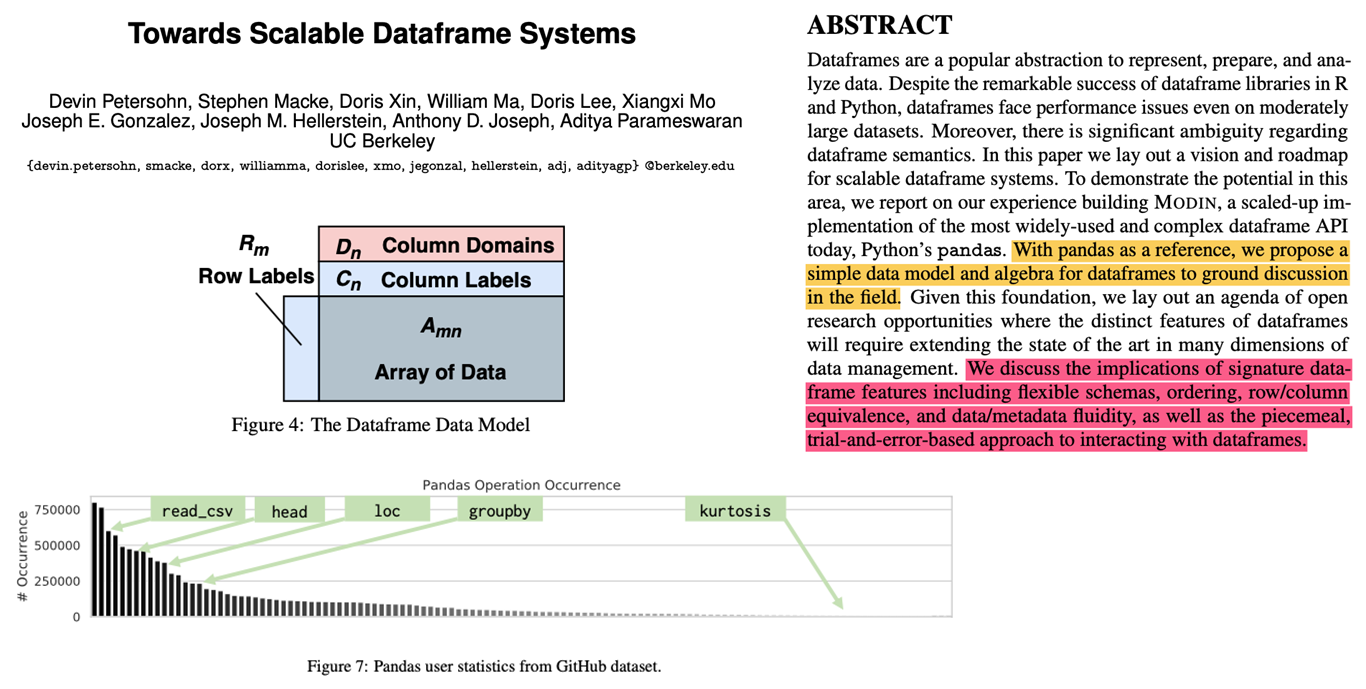
\includegraphics[scale=.33]{Bild3}\\
	       \url{https://arxiv.org/abs/2001.00888}
	\end{frame}
	
	
	\begin{frame}{Pandas Data Structures:Data Frames, Series, and Indices}
	    
	\end{frame}
	
	
	\begin{frame}{Pandas Data Structures }
	   There are three fundamental data structures in pandas:
	    \begin{itemize}
	        \item Data Frame: 2D data tabular data.
	        \item Series: 1D data. I usually think of it as columnar data.
	        \item Index: A sequence of row labels.
	    \end{itemize}
	    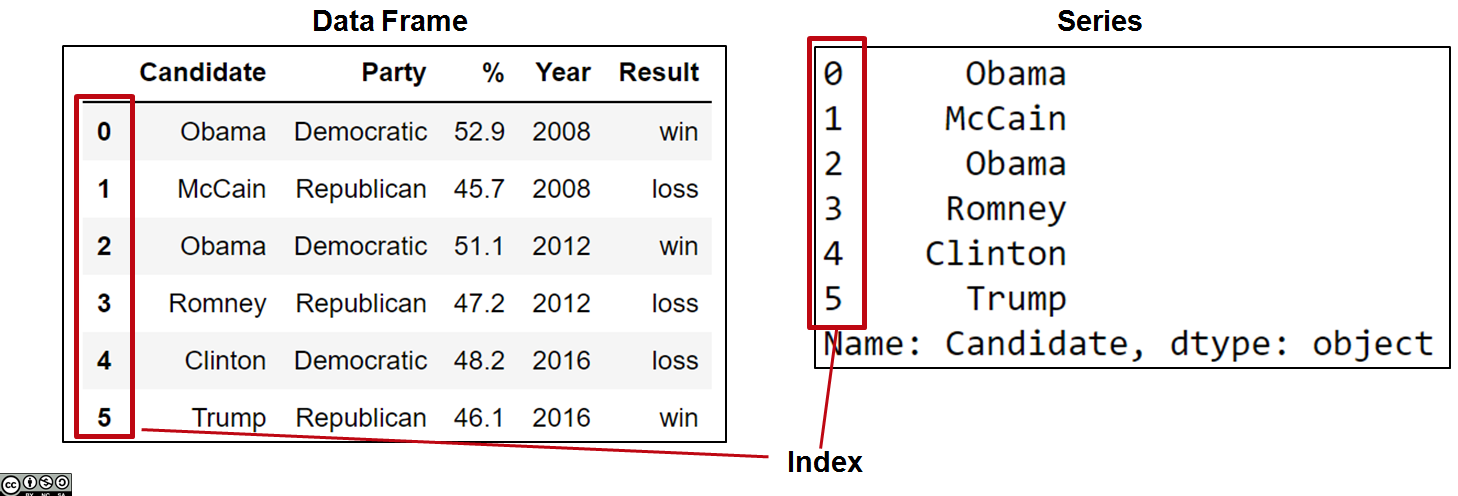
\includegraphics[scale=.36]{Bild4}
	\end{frame}
	
	
	\begin{frame}{The Relationship Between Data Frames, Series, and Indices }
	   We can think of a Data Frame as a collection of Series that all share the same Index
	    \begin{itemize}
	        \item Candidate, Party, \%, Year, and Result Series all share an index from  0 to 5.
	    \end{itemize}
	    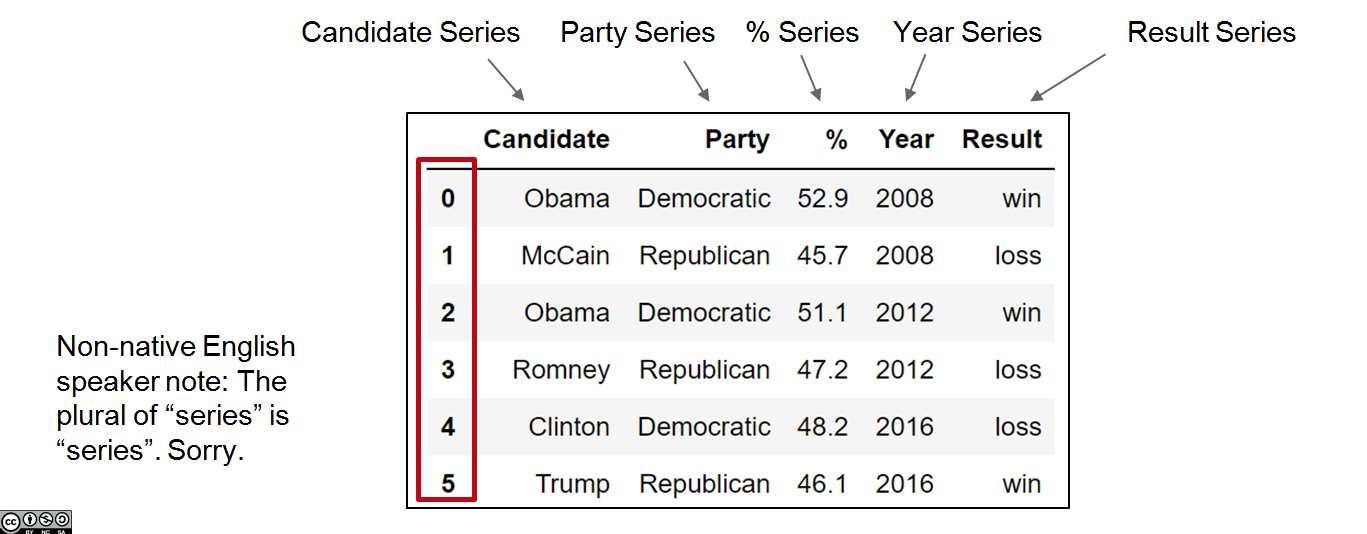
\includegraphics[scale=.39]{Bild5}
	\end{frame}
	
	
	\begin{frame}{Indices Are Not Necessarily Row Numbers}
	   Indices (a.k.a. row labels) can also:
	   \begin{itemize}
	       \item Be non-numeric.
	       \item Have a name, e.g. “State”. 
	   \end{itemize}
	    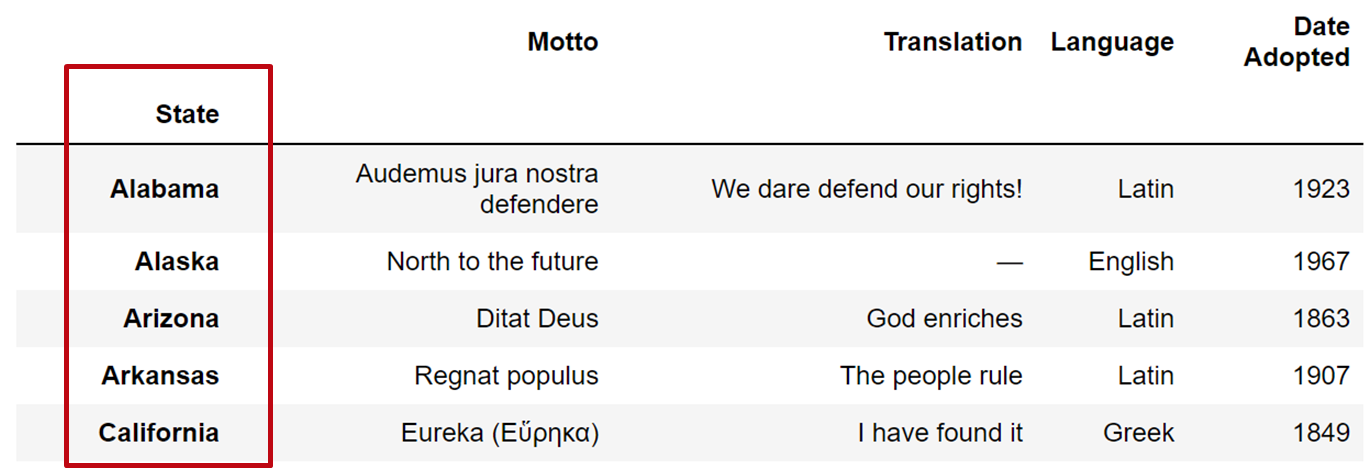
\includegraphics[scale=.39]{Bild6}
	\end{frame}
	
	
	\begin{frame}{Indices}
	   The row labels that constitute an index do not have to be unique
	   \begin{itemize}
	       \item Left: The index values are all unique and numeric, acting as a row number.
	       \item Right: The index values are named and non-unique.
	   \end{itemize}
	    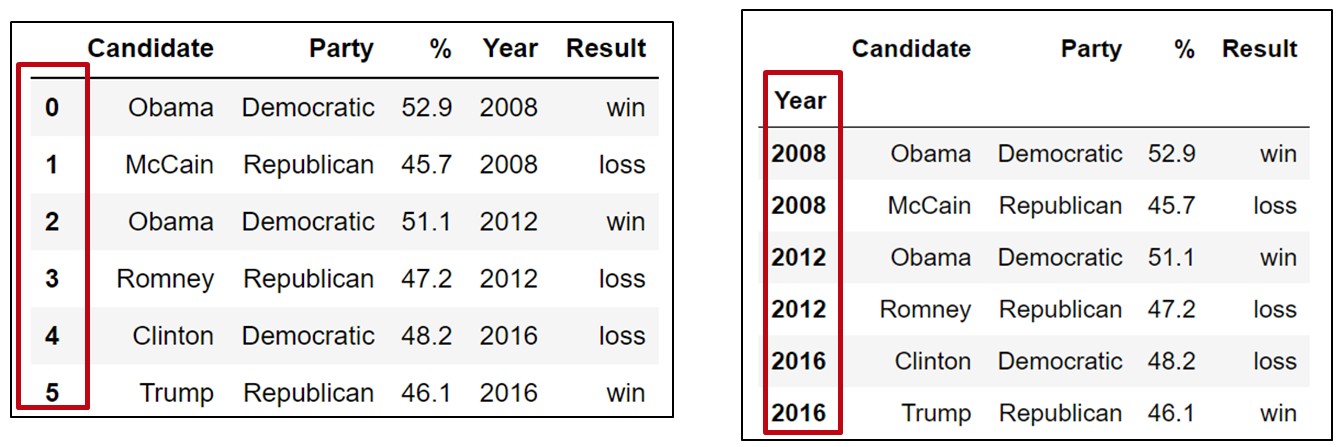
\includegraphics[scale=.39]{Bild7}
	\end{frame}
	
	
	
	\begin{frame}{Column Names Are Usually Unique!}
	   Column names in Pandas are almost always unique!
	   \begin{itemize}
	       \item Example: Really shouldn’t have two columns named “Candidate”. 
	   \end{itemize}
	   \centering
	    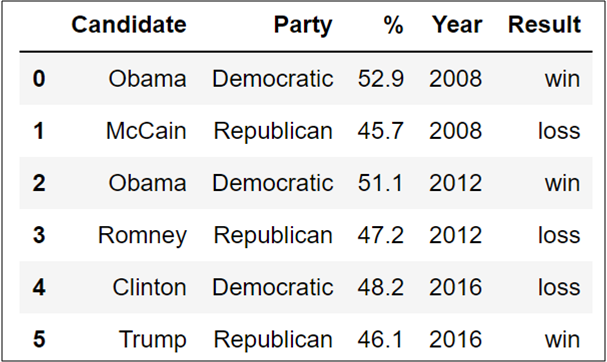
\includegraphics[scale=.75]{Bild8}
	\end{frame}
	
	
	\begin{frame}{Summary: structure of a Series}
	    \centering
	    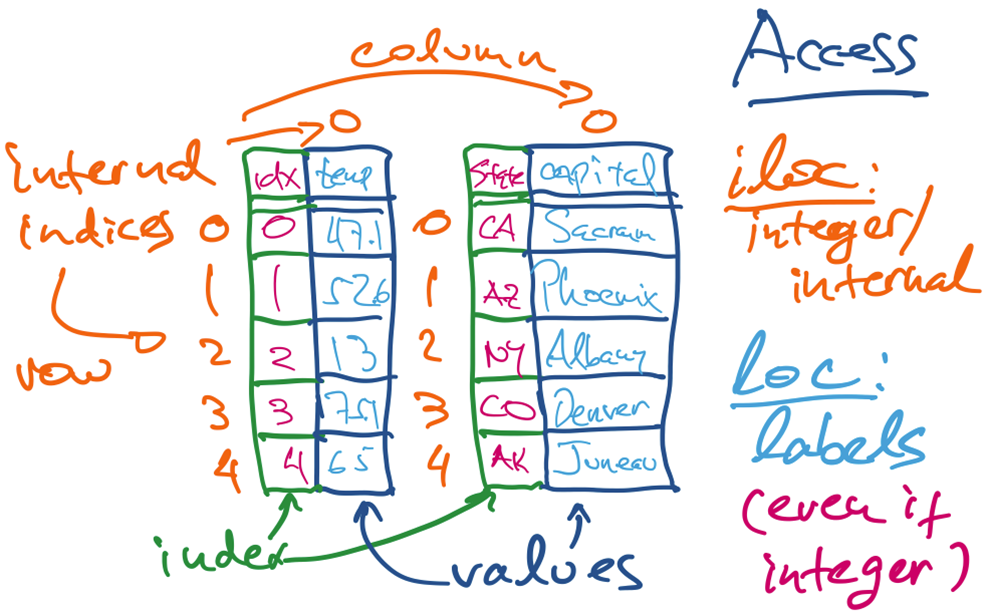
\includegraphics[scale=.5]{Bild9}
	\end{frame}
	
	\begin{frame}{Summary: structure of a DataFrame}
    	\centering
	    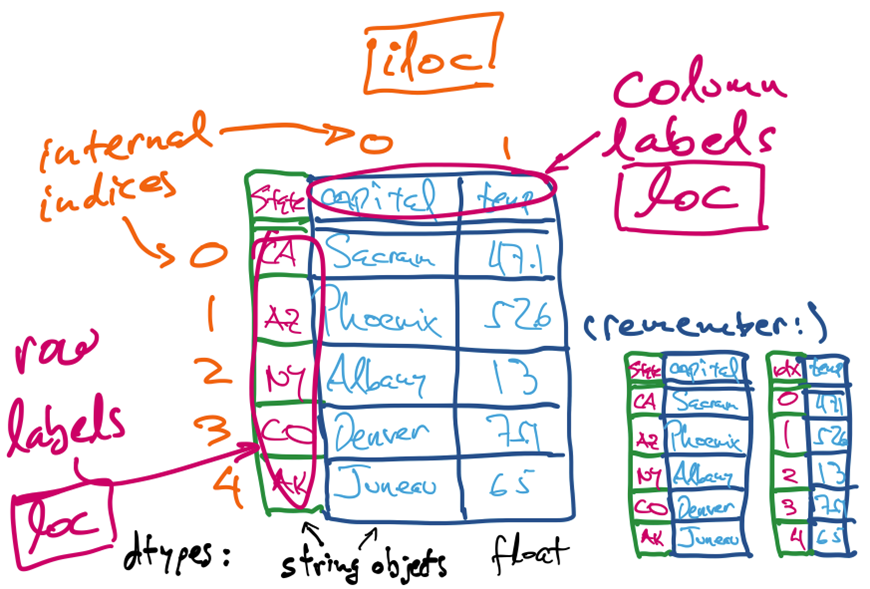
\includegraphics[scale=.5]{Bild10}
	\end{frame}
	
	\begin{frame}{Indexing with The [] Operator}

	\end{frame}
	
	
	\begin{frame}{Connecting with SQL: dataframes and relational ideas}
	       Given a dataframe, it is common to extract a Series or a collection of Series. This process is also known as “Column Selection” or sometimes “indexing by column”. 
	      \begin{columns}
	       
	        \begin{column}{.5\textwidth}
	            \begin{itemize}
	                \item Column name argument to [] yields Series.
	                \item List argument to [] yields a Data Frame.
	            \end{itemize}
	                  \begin{figure}
	                            
\includegraphics[scale=.3]{Bild11}  
	                  \end{figure}
	        \end{column}
	        
	        
	        \begin{column}{.5\textwidth}
	                  \begin{figure}
	                            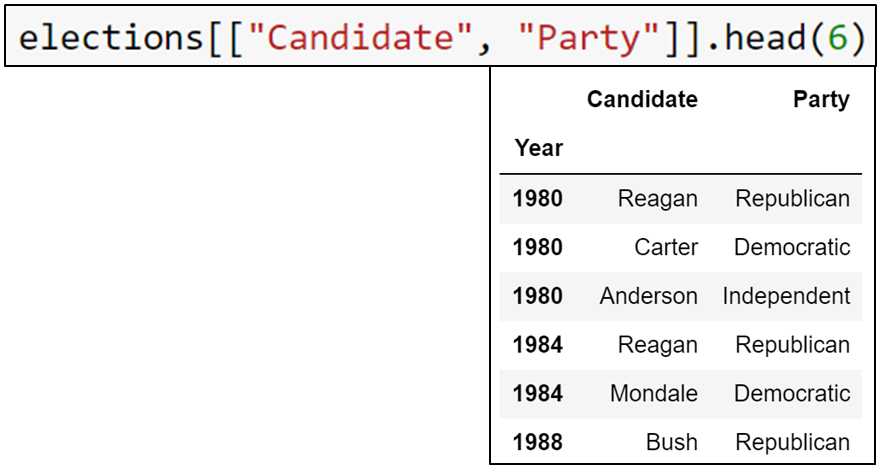
\includegraphics[scale=.3]{Bild12}  
	                  \end{figure}
	        \end{column}
	      \end{columns}
	\end{frame}
	
	
	\begin{frame}{Indexing by Column Names Using [] Operator}
	       Given a dataframe, it is common to extract a Series or a collection of Series. This process is also known as “Column Selection” or sometimes “indexing by column”. 
	      \begin{columns}
	       
	        \begin{column}{.5\textwidth}
	            \begin{itemize}
	                \item Column name argument to [] yields Series.
	                \item List argument (even of one name) to [] yields a Data Frame.
	            \end{itemize}
	                  \begin{figure}
	                            
\includegraphics[scale=.3]{Bild11}  
	                  \end{figure}
	        \end{column}
	        
	        
	        \begin{column}{.5\textwidth}
	                  \begin{figure}
	                            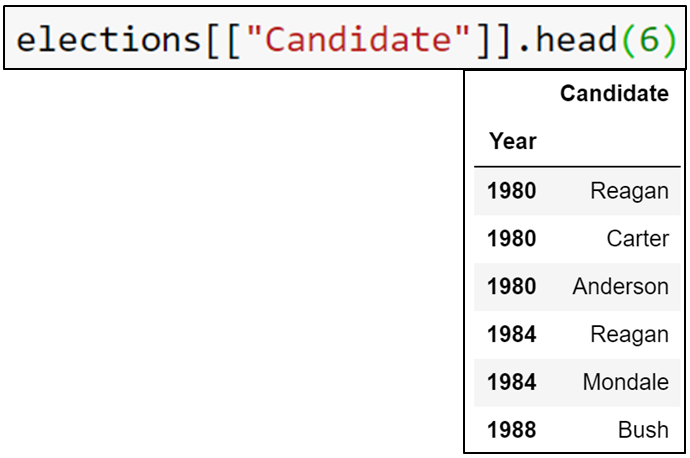
\includegraphics[scale=.3]{Bild13}  
	                  \end{figure}
	        \end{column}
	      \end{columns}
	\end{frame}
	
	
	
	\begin{frame}{Indexing by Row Slices Using [] Operator}
        We can also index by row numbers using the [] operator. 
        \begin{itemize}
            \item Numeric slice argument to [] yields rows.
            \item Example: [0:3] yields rows 0 to 2.
        \end{itemize}
    
    	\centering
	    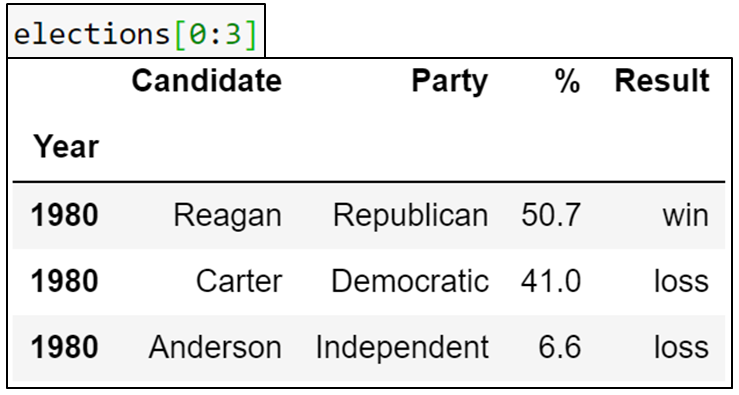
\includegraphics[scale=.5]{Bild14}
	\end{frame}
	
	
	
	\begin{frame}{[] Summary}
    	\centering
	    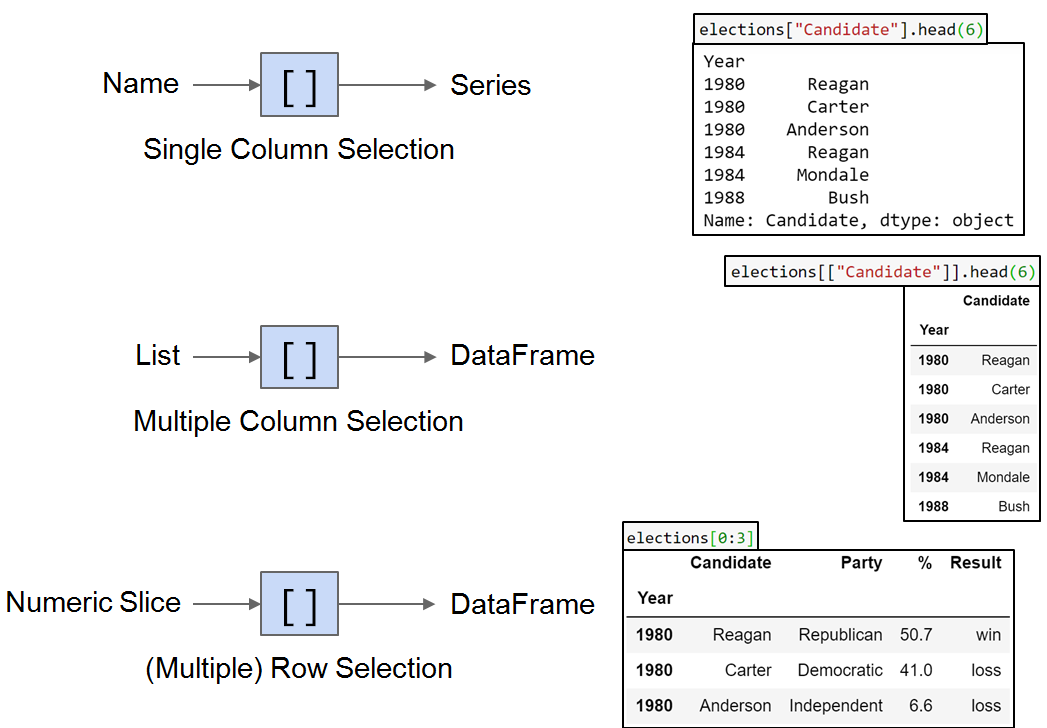
\includegraphics[scale=.33]{Bild15}
	\end{frame}
	
	\begin{frame}{Question}
	   \begin{columns}
	        \begin{column}{.5\textwidth}
    	         \begin{figure}

    	            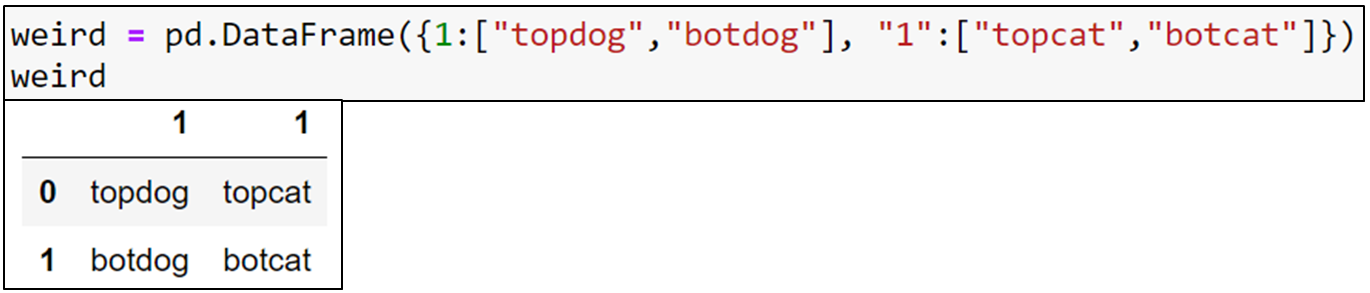
\includegraphics[scale=.35]{Bild17}
    	        \end{figure} 
    	        Try to predict the output of the following:
	          \begin{itemize}
	              \item weird[1]
	              \item weird[“1”]
	              \item weird[1:]
	          \end{itemize}
	        \end{column}
	        \begin{column}{.3\textwidth}
	        \bigskip
	        \bigskip
	        \bigskip
	        \begin{figure}
	              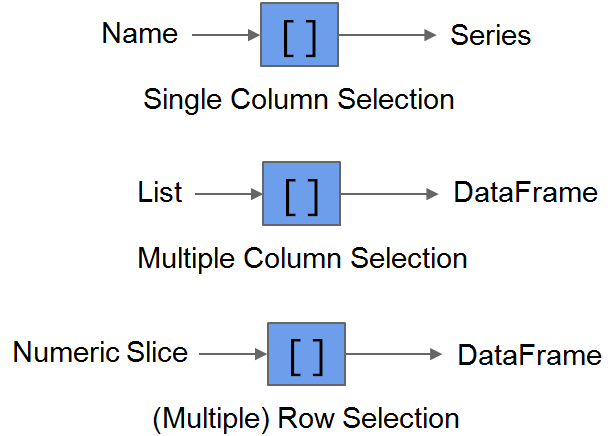
\includegraphics[scale=.35]{Bild16}
	        \end{figure}
	              
	        \end{column}
	   \end{columns}     
	\end{frame}

	
	\begin{frame}{Boolean Array Selection and Querying}
	    
	\end{frame}
	
	
	\begin{frame}{Boolean Array Input}
	    Yet another input type supported by [] is the boolean array.\\
	    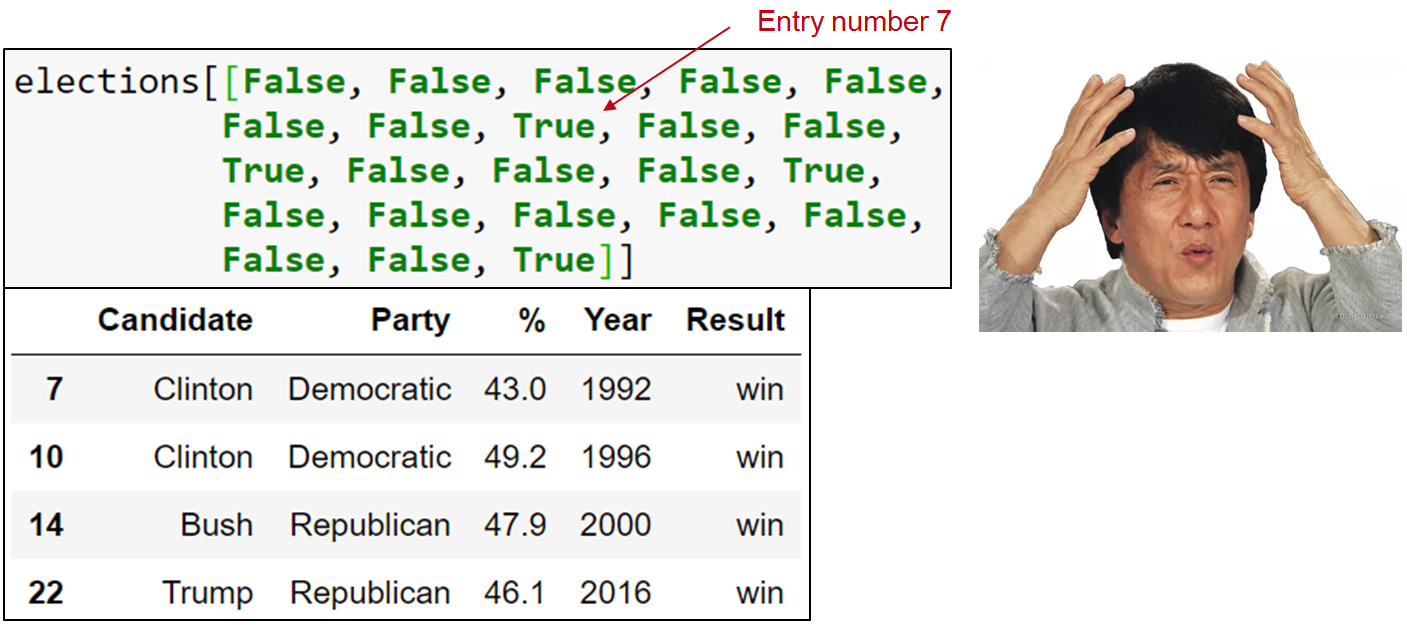
\includegraphics[scale=.35]{Bild18}
	\end{frame}
	
	
	\begin{frame}{Boolean Array Input}
	   Yet another input type supported by [] is the boolean array. Useful because boolean arrays can be generated by using logical operators on Series.
	    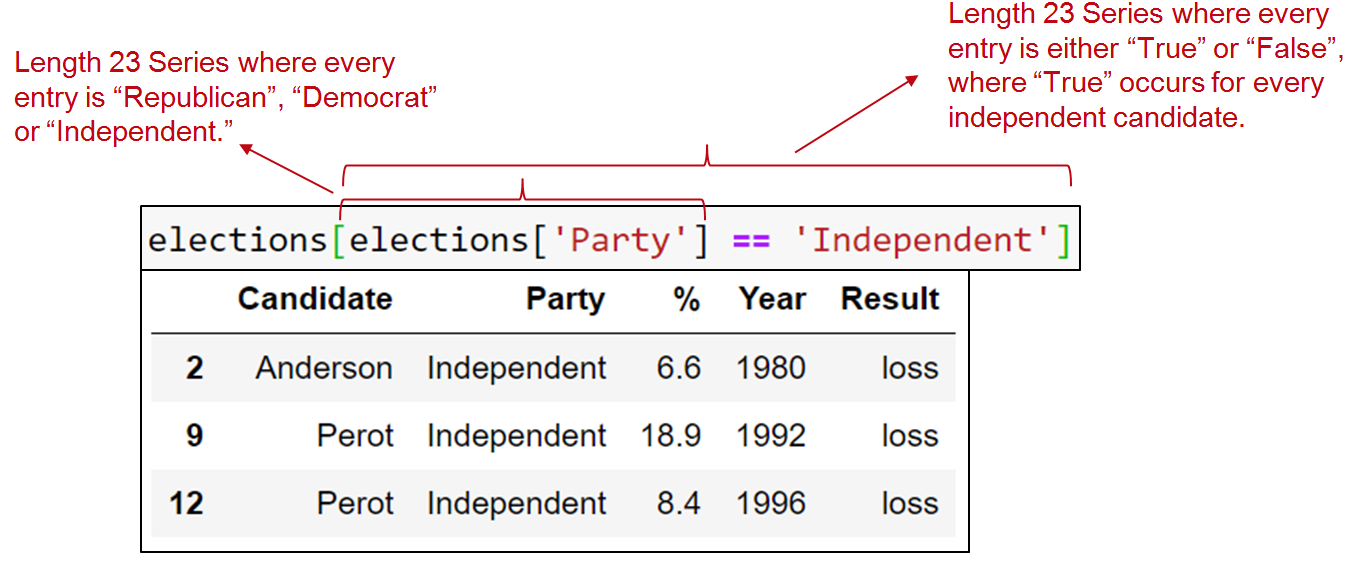
\includegraphics[scale=.35]{Bild19}
	\end{frame}
	
	
	\begin{frame}{Boolean Array Input}
	    \centering
	   Boolean Series can be combined using the & operator, allowing filtering of results by multiple criteria.
	    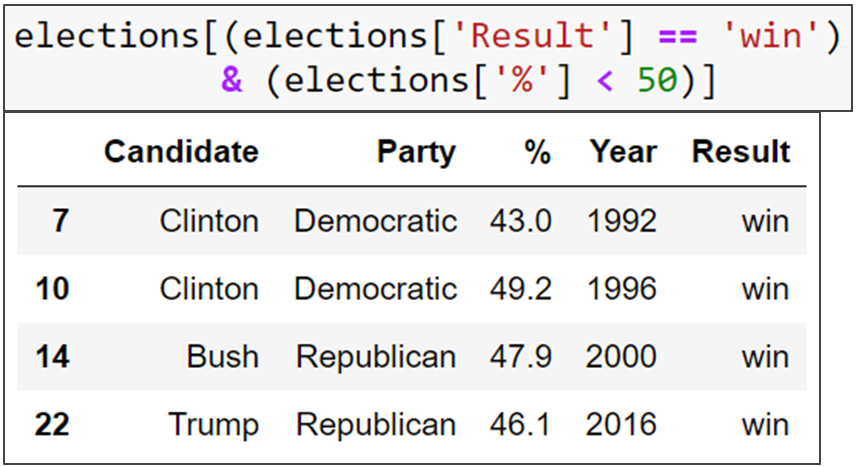
\includegraphics[scale=.5]{Bild20}
	\end{frame}
	
	
	\begin{frame}{isin}
	    The isin function makes it more convenient to find rows that match one of many possible values.\\
	    \bigskip

	  Example: Suppose we want to find “Republican” or “Democratic” candidates. Could use the | operator (| means or), or we can use isin.
	  \begin{itemize}
	      \item Ugly:
	  \end{itemize}
	    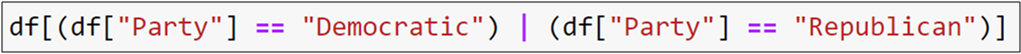
\includegraphics[scale=.5]{Bild21}
	    \begin{itemize}
	        \item Better:
	    \end{itemize}
	    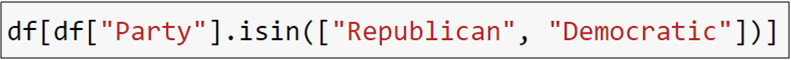
\includegraphics[scale=.5]{Bild22}
	\end{frame}
	
	\begin{frame}{The Query Command}

	  The query command provides an alternate way to combine multiple conditions
	  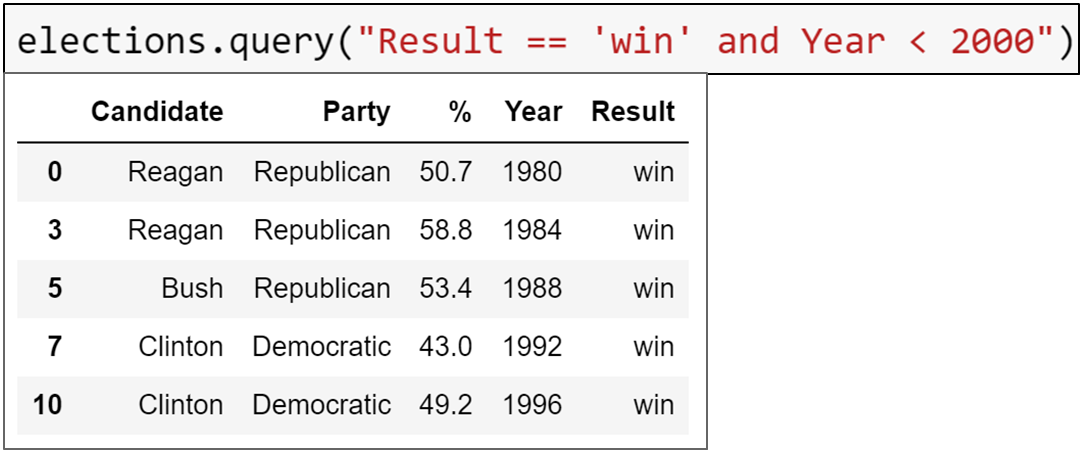
\includegraphics[scale=.5]{Bild23}
	\end{frame}
	
	\begin{frame}{Indexing with .loc and .iloc
Sampling with .sample}

	\end{frame}
	
	
	\begin{frame}{Loc and iloc}
	    Loc and iloc are alternate ways to index into a DataFrame.
	    \begin{itemize}
	        \item They take a lot of getting used to! Documentation and ideas behind them are quite complex.
	        \item I’ll go over common usages (see docs for weirder ones).
	    \end{itemize}
	    Documentation:
	    \begin{itemize}
	        \item loc: \url{https://pandas.pydata.org/pandas-docs/stable/generated/pandas.DataFrame.loc.html}
	        \item iloc:  \url{https://pandas.pydata.org/pandas-docs/stable/generated/pandas.DataFrame.iloc.html}
	        \item More general docs on indexing and selecting
	    \end{itemize}
	\end{frame}
	
	
	\begin{frame}{Loc}
	    Loc does two things:
	    \begin{itemize}
	        \item Access values by labels.
	        \item Access values using a boolean array (a la Boolean Array Selection).
	    \end{itemize}
	\end{frame}
	
	
	\begin{frame}{Loc with Lists}
	    The most basic use of loc is to provide a list of row and column labels, which returns a DataFrame
	    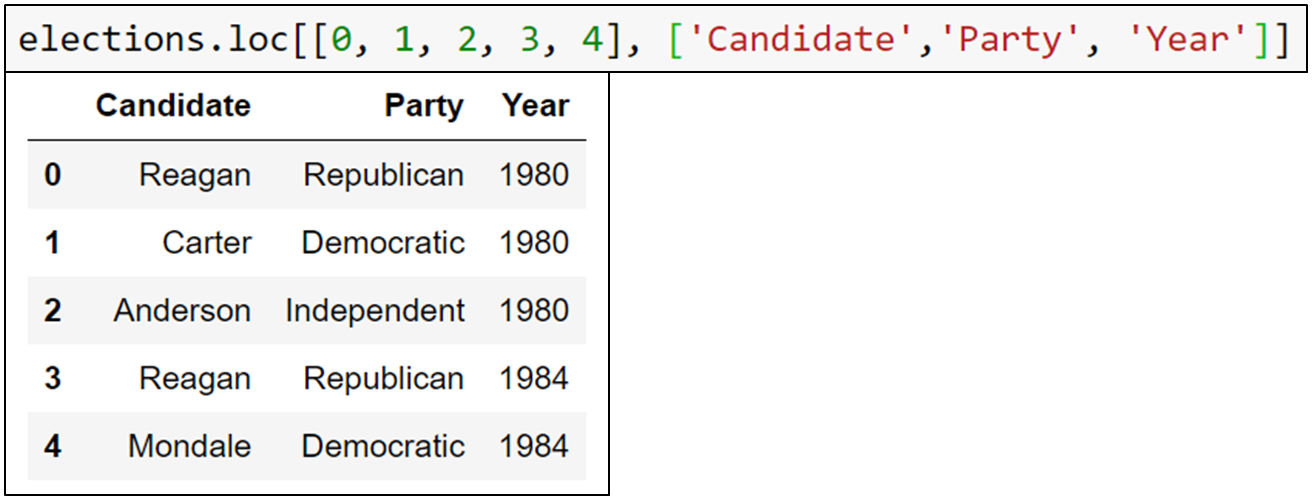
\includegraphics[scale=.43]{Bild24}
	\end{frame}
	
	\begin{frame}{Loc with Lists}
	    The most basic use of loc is to provide a list of row and column labels, which returns a DataFrame
	    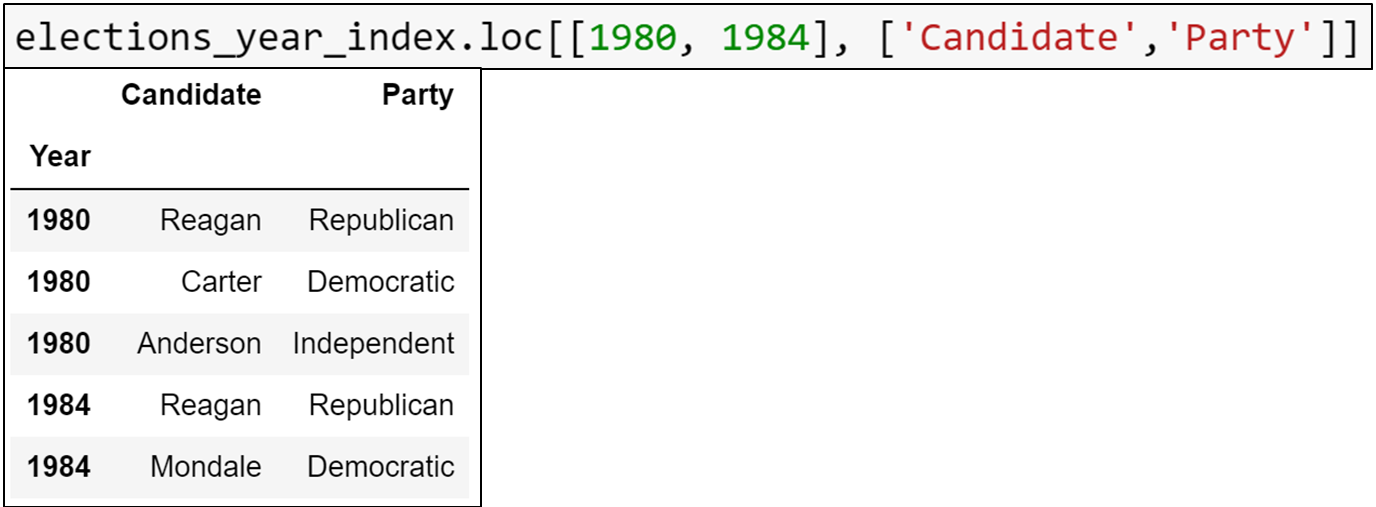
\includegraphics[scale=.42]{Bild25}
	\end{frame}
	
	
	\begin{frame}{Loc with Slices}
	    Loc is also commonly used with slices
	    \begin{itemize}
	        \item Slicing works with all label types, not just numeric labels.
	        \item Slices with loc are inclusive, not exclusive.
	    \end{itemize}
	    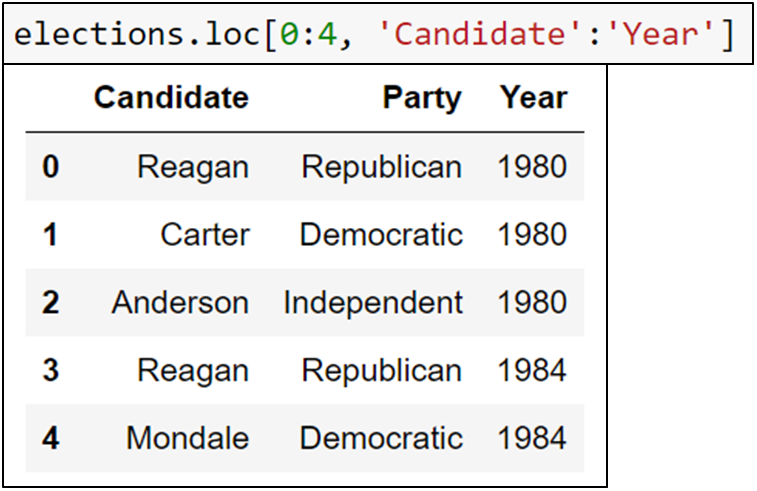
\includegraphics[scale=.4]{Bild26}
	\end{frame}
	
	
	\begin{frame}{Loc with Slices}
	    Loc is also commonly used with slices
	    \begin{itemize}
	        \item Slicing works with all label types, not just numeric labels.
	        \item Slices with loc are inclusive, not exclusive.
	    \end{itemize}
	    
\includegraphics[scale=.39]{Bild27}
	\end{frame}
	
	
	\begin{frame}{Loc with Single Values for Column Label}
	   If we provide only a single label as column argument, we get a Series.
	    
\includegraphics[scale=.5]{Bild28}
	\end{frame}
	
	
	\begin{frame}{Loc with Single Values for Column Label}
	   As before with the [] operator, if we provide a list of only one label as an argument, we get back a dataframe.
	    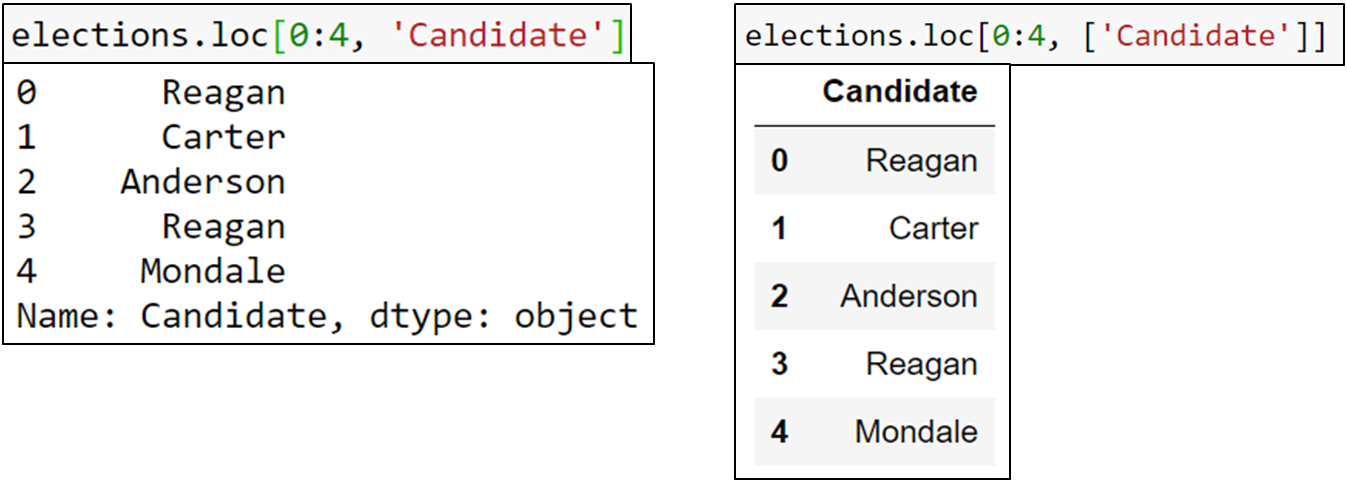
\includegraphics[scale=.4]{Bild29}
	\end{frame}
	
	\begin{frame}{Loc with Single Values for Row Label}
	   If we provide only a single row label, we get a Series.
	   \begin{itemize}
	       \item Such a series represents a ROW not a column!
	       \item The index of this Series is the names of the columns from the data frame.
	       \item Putting the single row label in a list yields a dataframe version.
	   \end{itemize}
	    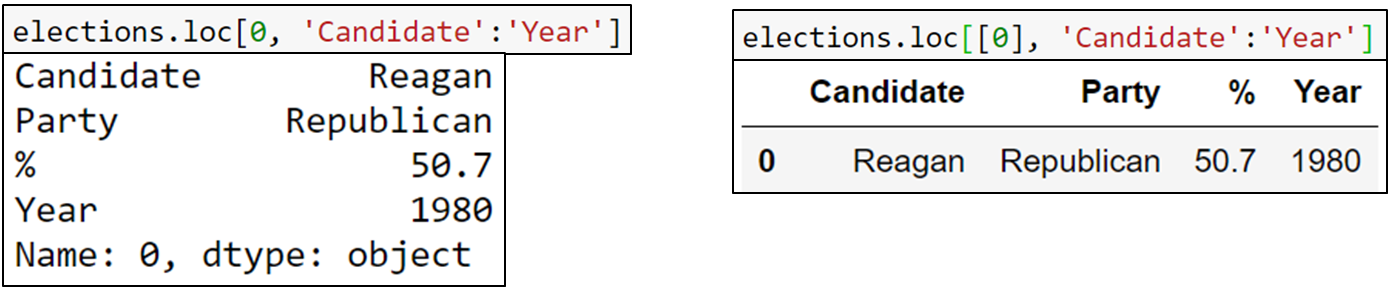
\includegraphics[scale=.4]{Bild30}
	\end{frame}
	
	
	\begin{frame}{Loc Supports Boolean Arrays}
	   Loc supports Boolean Arrays exactly as you’d expect.
	    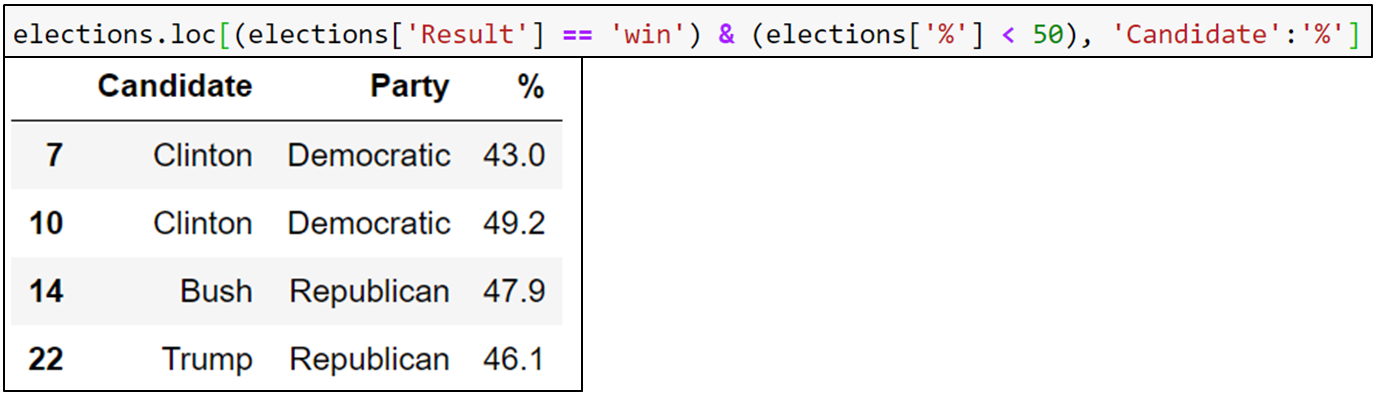
\includegraphics[scale=.4]{Bild31}
	\end{frame}
	
	
	\begin{frame}{iloc: Integer-Based Indexing for Selection by Position}
	   In contrast to loc, iloc doesn’t think about labels at all. Instead, it returns the items that appear in the numerical positions specified.
	    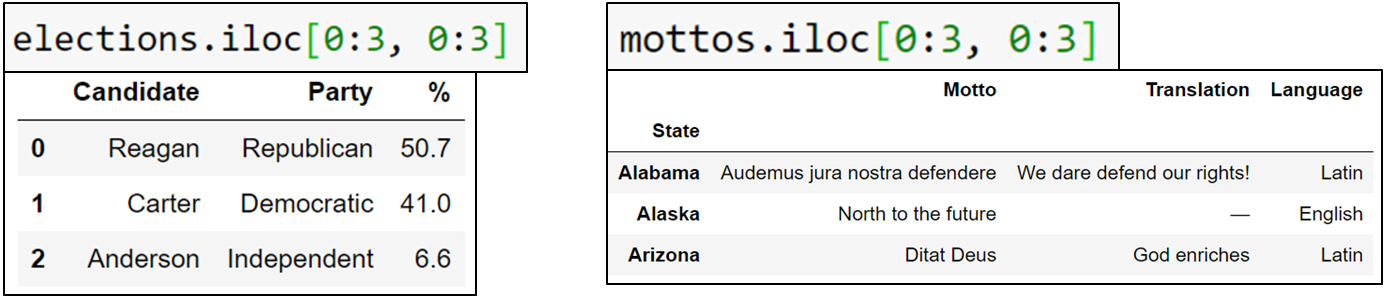
\includegraphics[scale=.4]{Bild32}
	    Advantages of loc:
	    \begin{itemize}
	        \item Harder to make mistakes.
	        \item Easier to read code.
	        \item Not vulnerable to changes to the ordering of rows/cols in raw data files.
	    \end{itemize}
	    Nonetheless, iloc can be more convenient. Use iloc judiciously
	\end{frame}
	
	
	\begin{frame}{Annoying Question Challenge }
	   Which of the following pandas statements returns a DataFrame of the first 3 Candidate names only for candidates that won with more than 50\% of the vote.
	   
	   elections.iloc[[0, 3, 5], [0, 3]]\\
       elections.loc[[0, 3, 5], ["Candidate":"Year"]\\
       elections.loc[elections["\%"] > 50, ["Candidate", "Year"]].head(3)\\
       elections.loc[elections["\%"] > 50, ["Candidate", "Year"]].iloc[0:2, :]\\

	    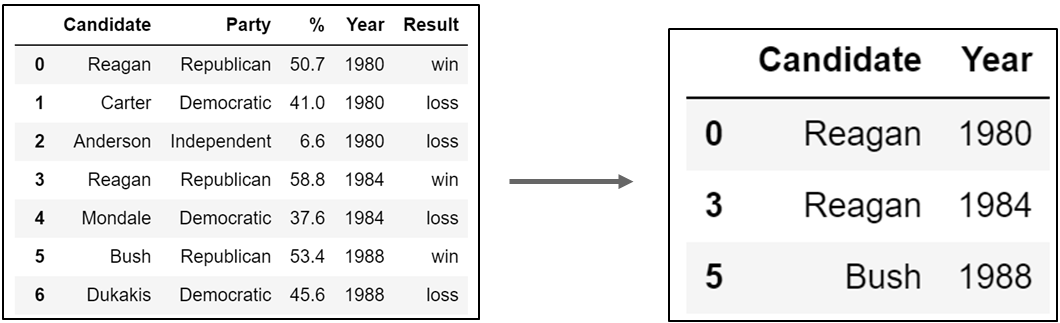
\includegraphics[scale=.4]{Bild33}
	\end{frame}
	
	\begin{frame}{Annoying Question Challenge }
	   Which of the following pandas statements returns a DataFrame of the first 3 Candidate names only for candidates that won with more than 50\% of the vote.
	   
	   \textbf{elections.iloc[[0, 3, 5], [0, 3]]}\\
       elections.loc[[0, 3, 5], ["Candidate":"Year"]\\
       \textbf{elections.loc[elections["\%"] > 50, ["Candidate", "Year"]].head(3)}\\
       elections.loc[elections["\%"] > 50, ["Candidate", "Year"]].iloc[0:2, :]\\

	    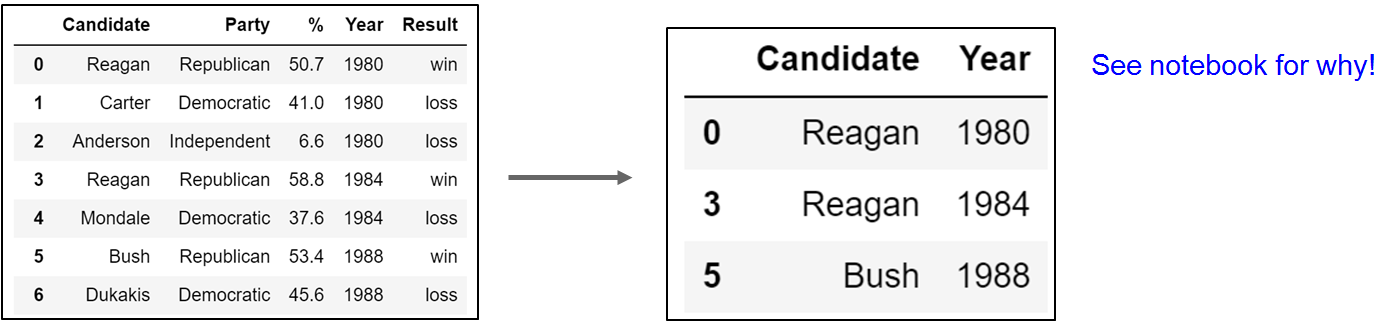
\includegraphics[scale=.4]{Bild34}
	\end{frame}
	
	
	\begin{frame}{Note on Exam Problems}
	   Q: Are you going to put horrible problems like these on the exam?
	   
	   A: Technically such problems would be in scope, but it’s very unlikely they’ll be this nitpicky.

	    
\includegraphics[scale=.5]{Bild35}
	\end{frame}
	
	
	\begin{frame}{Sample}
	   If you want a DataFrame consisting of a random selection of rows, you can use the sample method.
	   \begin{itemize}
	       \item By default, it is without replacement. Use replace=true for replacement.
	       \item Naturally, can be chained with our selection operators [], loc, iloc.
	   \end{itemize}
	    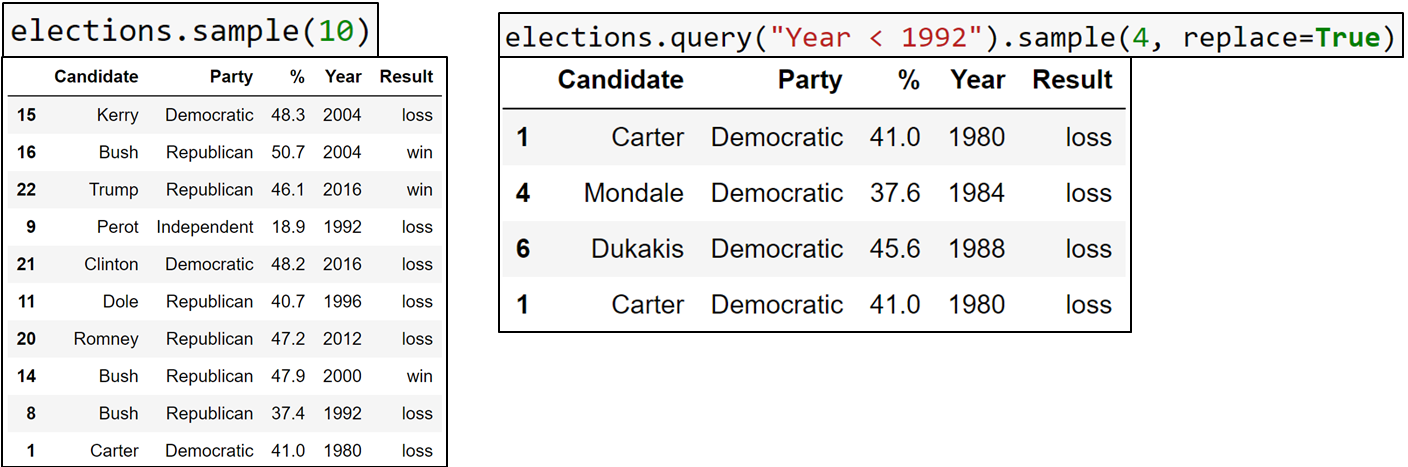
\includegraphics[scale=.4]{Bild36}
	\end{frame}
	
	
	\begin{frame}{Handy Properties and Utility Functions for Series and DataFrames}
	    
	\end{frame}
	
	
	
	\begin{frame}{Numpy Operations}
	   Pandas Series and DataFrames support a large number of operations, including mathematical operations so long as the data is numerical.
	    \includegraphics[scale=.4]{Bild37}
	\end{frame}
	
	
	\begin{frame}[c]{head, size, shape, and describe}
	    head: Displays only the top few rows.\\
        size: Gives the total number of data points.\\
        shape: Gives the size of the data in rows and columns.\\
        describe: Provides a summary of the data.\\

	\end{frame}
	
	
	\begin{frame}[c]{index and columns}
	    index: Returns the index (a.k.a. row labels).\\
        columns: Returns the labels for the columns.
	\end{frame}
	
	
	\begin{frame}{The sort\_values Method}
	   One incredibly useful method for DataFrames is sort\_values, which creates a copy of a DataFrame sorted by a specific column.\\
	    \includegraphics[scale=.4]{Bild38}
	\end{frame}
	
	
	
	\begin{frame}{The sort\_values Method}
	   We can also use sort\_values on a Series, which returns a copy with with the values in order.\\
	    \includegraphics[scale=.5]{Bild39}
	\end{frame}
	
	\begin{frame}{The value\_counts Method}
	   Series also has the function value\_counts, which creates a new Series showing the counts of every value\\
	    \includegraphics[scale=.6]{Bild40}
	\end{frame}
	
	
	\begin{frame}{The unique Method}
	   Another handy method for Series  is unique, which returns all unique values as an array.\\
	    \includegraphics[scale=.4]{Bild41}
	\end{frame}
	
	
	\begin{frame}{The Things We Just Saw}
	    \begin{itemize}
	        \item sort\_values
	        \item value\_counts
	        \item unique
	    \end{itemize}
	\end{frame}
	
	
	\begin{frame}{Baby Names Exploration}
	    
	\end{frame}
	
	
	\begin{frame}[c]{Wrapping Up}
	    To wrap up today, let’s try answering some questions about a list of California baby names.
	    
	    I’ll start with my own goal, and will then take suggested goals from you and try to write code to achieve your goals.

	\end{frame}
\end{document}